\documentclass[11pt,a4paper]{article} 
\usepackage[font={footnotesize,it}]{caption}
\usepackage{latexsym}
\usepackage{amsmath}
\usepackage{amssymb}
\usepackage{dsfont}
\usepackage{tikz}
\usepackage{listings}
\usepackage{ifthen}
\usepackage{paralist}
\usepackage{enumitem}

\parskip        0mm
\oddsidemargin  0in
\evensidemargin 0in
\textwidth      6in
\topmargin      0in
\marginparwidth 30pt
\textheight     9.2in
\headheight     .1in
\headsep        .1mm

\lstset{
  basicstyle=\footnotesize\ttfamily,
  numbers=left,
  numberstyle=\tiny,
  numbersep=10pt,
  tabsize=4,
  extendedchars=true,
  breaklines=true,
  keywordstyle=\ttfamily,
  stringstyle=\ttfamily,
  showspaces=false,
  showtabs=false,
  xleftmargin=17pt,
  framexleftmargin=17pt,
  framexrightmargin=5pt,
  framexbottommargin=4pt,
  showstringspaces=false   
}
\lstloadlanguages{ 
  C , C++, ml
}

\title{VU Parallel Computing\\ 
\Large Project Report}
\author{Name: \underline{Stefan Marschner, Moritz Macke}\qquad
  Matr. number: \underline{1426962, 0327088}}
\date{Due: June 19, 2017}


\begin{document}

\maketitle
\section{Abstract}

We present three different implementations of a parallelized Quicksort algorithm in MPI, Cilk and OpenMP. By testing the implementations on multi-core systems we aim to compare the different algorithms in terms of runtime.

\section{OpenMP}
\subsection{Algorithm}
\subsection{Analysis}
\section{Cilk}
\subsection{Algorithm}
\subsection{Analysis}
\section{MPI}
\subsection{Algorithm}
\begin{figure}[h]
	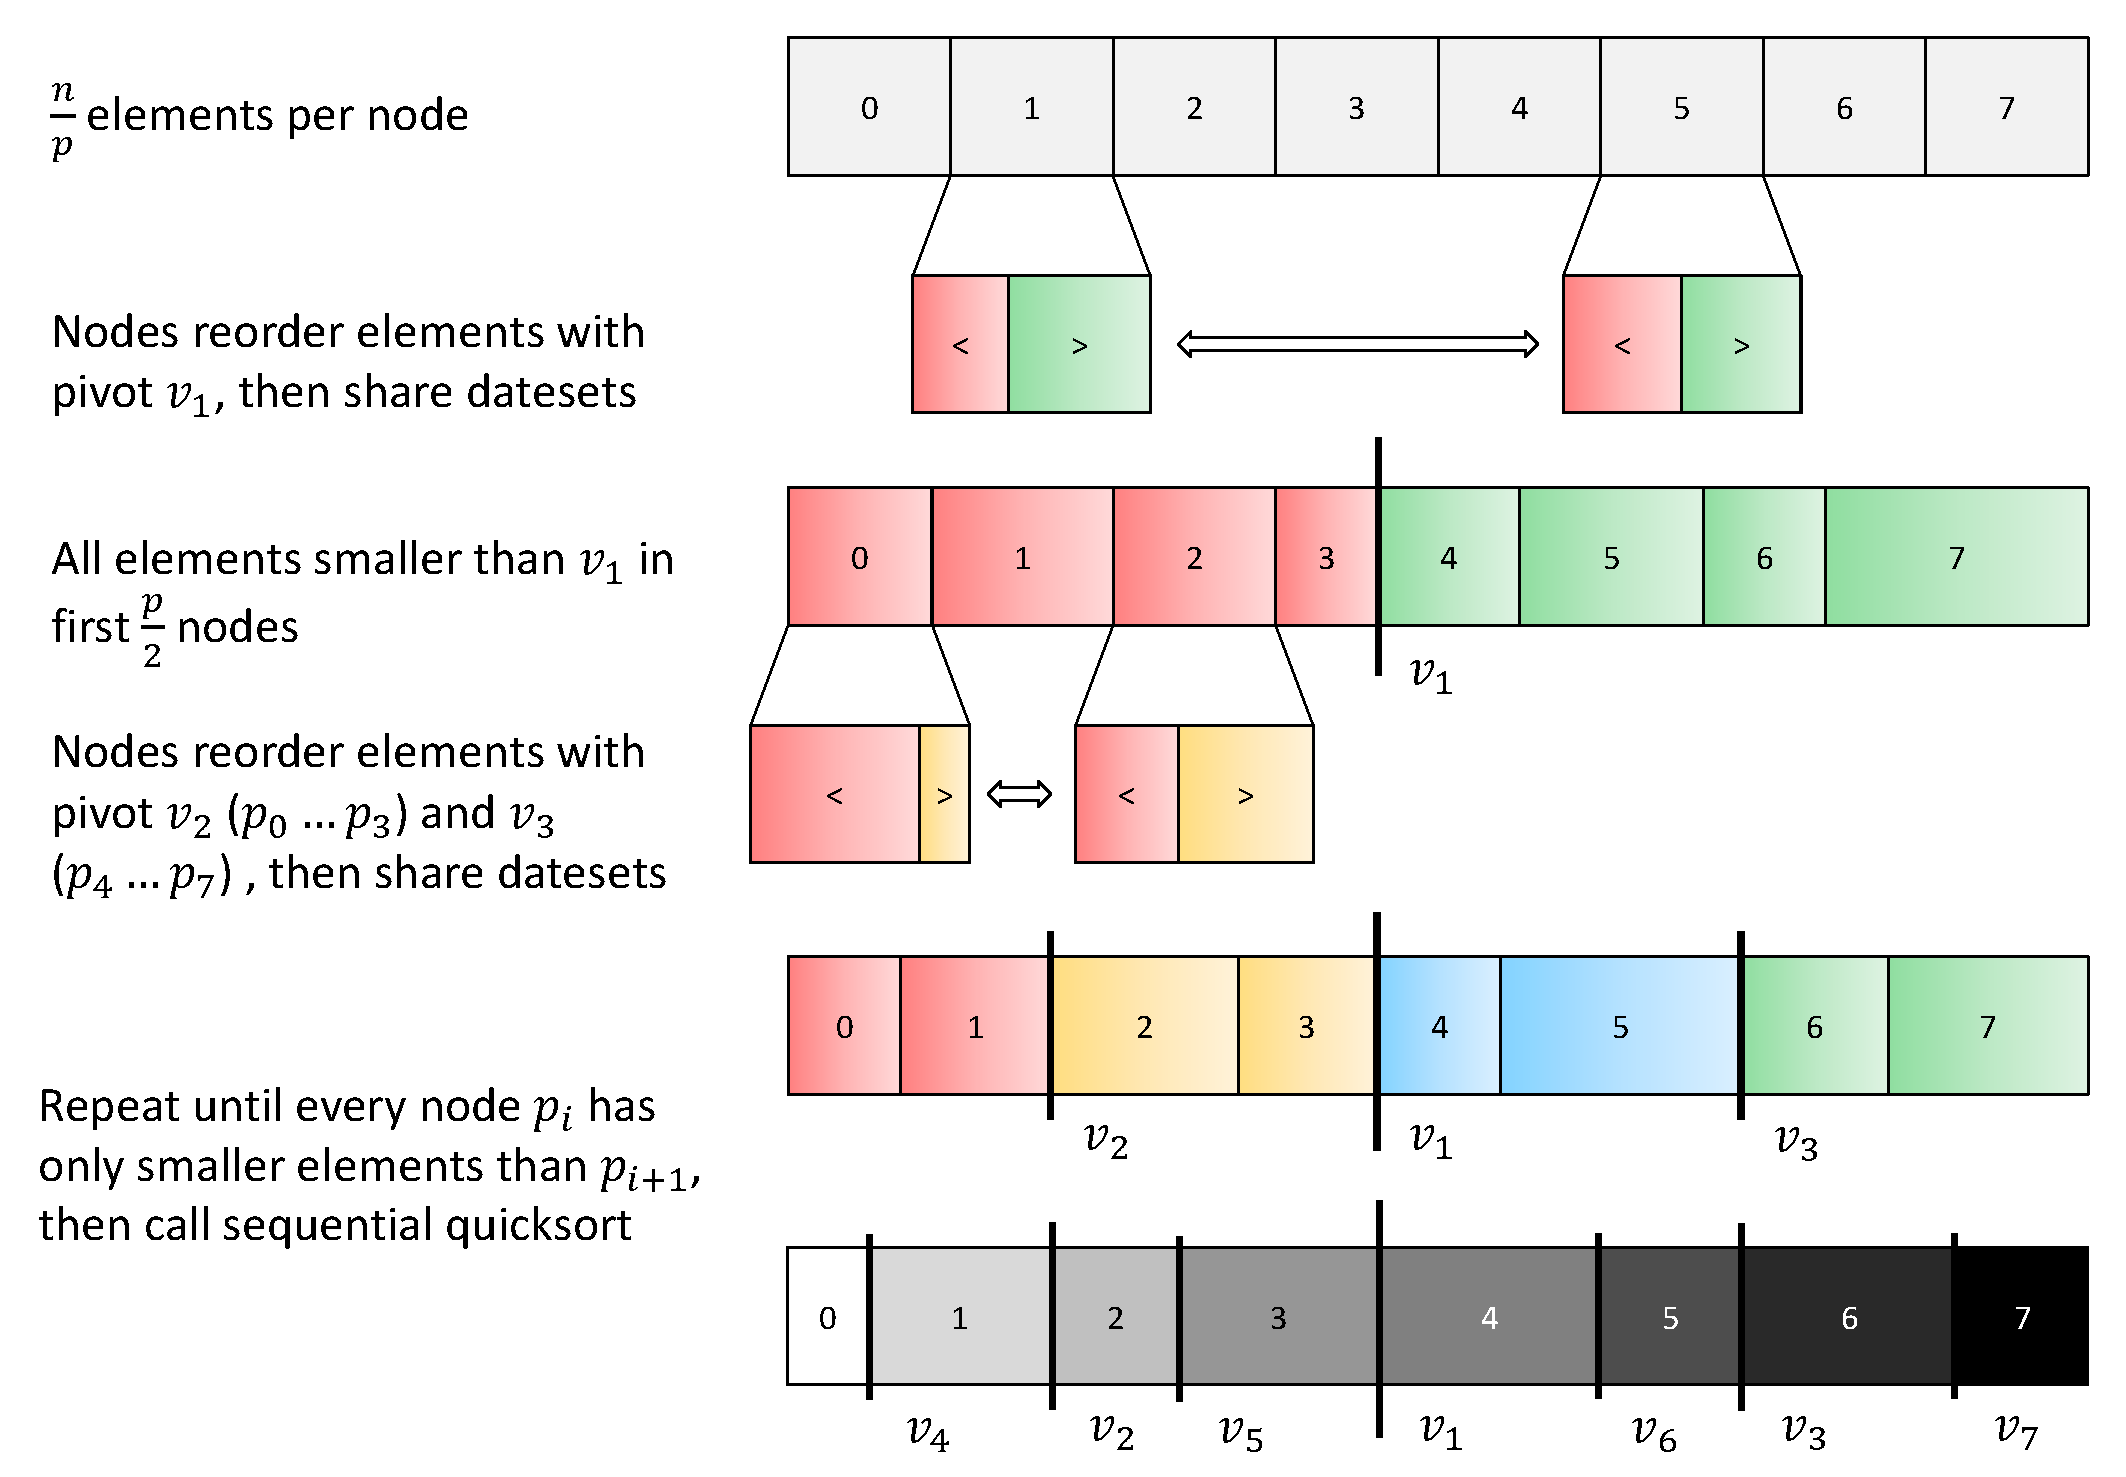
\includegraphics[width=\textwidth]{img/mpi_algorithm.pdf}
	\caption{Example of the partitioning for the parallel Quicksort implementation for p = 8.}
\end{figure}
\begin{enumerate}
	\item Divide input into (roughly) $\frac{n}{p}$ elements per node.
	\item Node 0 is arbitrarily chosen as "master", all others as "slave".
	\item At the start, all node are part of the same "set" (sets are emphasized by different colors in the graphic).
	\item Every node picks 5 elements at random and computes median, then sends it to the master.
	\item Master chooses pivots for every set of nodes and sends it to them.
	\item Every node reorders their dataset using the received pivot.
	\item Depending on their rank, all nodes send and receive part of a dataset to/from another node so that the lower $\frac{p}{2}$ nodes only have elements smaller than the pivot and the higher $\frac{p}{2}$ nodes only have elements bigger than the pivot.
	\item Every set of nodes is split in half and steps 4-7 are repeated until every node is in its own set.
	\item A sequential Quicksort implementation is called in every node.
	\item Every slave sends its sorted dataset to the master, which reassembles the datasets into the full sorted array.
	
\end{enumerate}
\subsection{Analysis}

\textbf{Drawbacks}\newline
The implementation works best for randomized input. If the array is pre-sorted, it would have a significant negative effect on the runtime of the algorithm because most of the work would be done by a single node. "Rebalancing" the datasets for a better utilization of all nodes would be difficult and may not necessarily improve runtime. 

\section{Test System}

\section{Test Results}
\subsection{MPI}
\textbf{Pivot Selection}\newline
As noted above, in our implementation the median of 5 random elements is sent to the master, which calculates the median of all received pivots from a set of processors and sends this new pivot back to the set of processors. We tested our implementation with $n=10^{8}$ and different numbers of elements randomly selected for the calculation of the pivot. We also tested the case that the pivot is always 0. This is the worst case scenario in which every element is received by processor 0 and the algorithm degenerates into sequential Quicksort with the additional overhead of the partitioning.
\begin{figure}[h]
	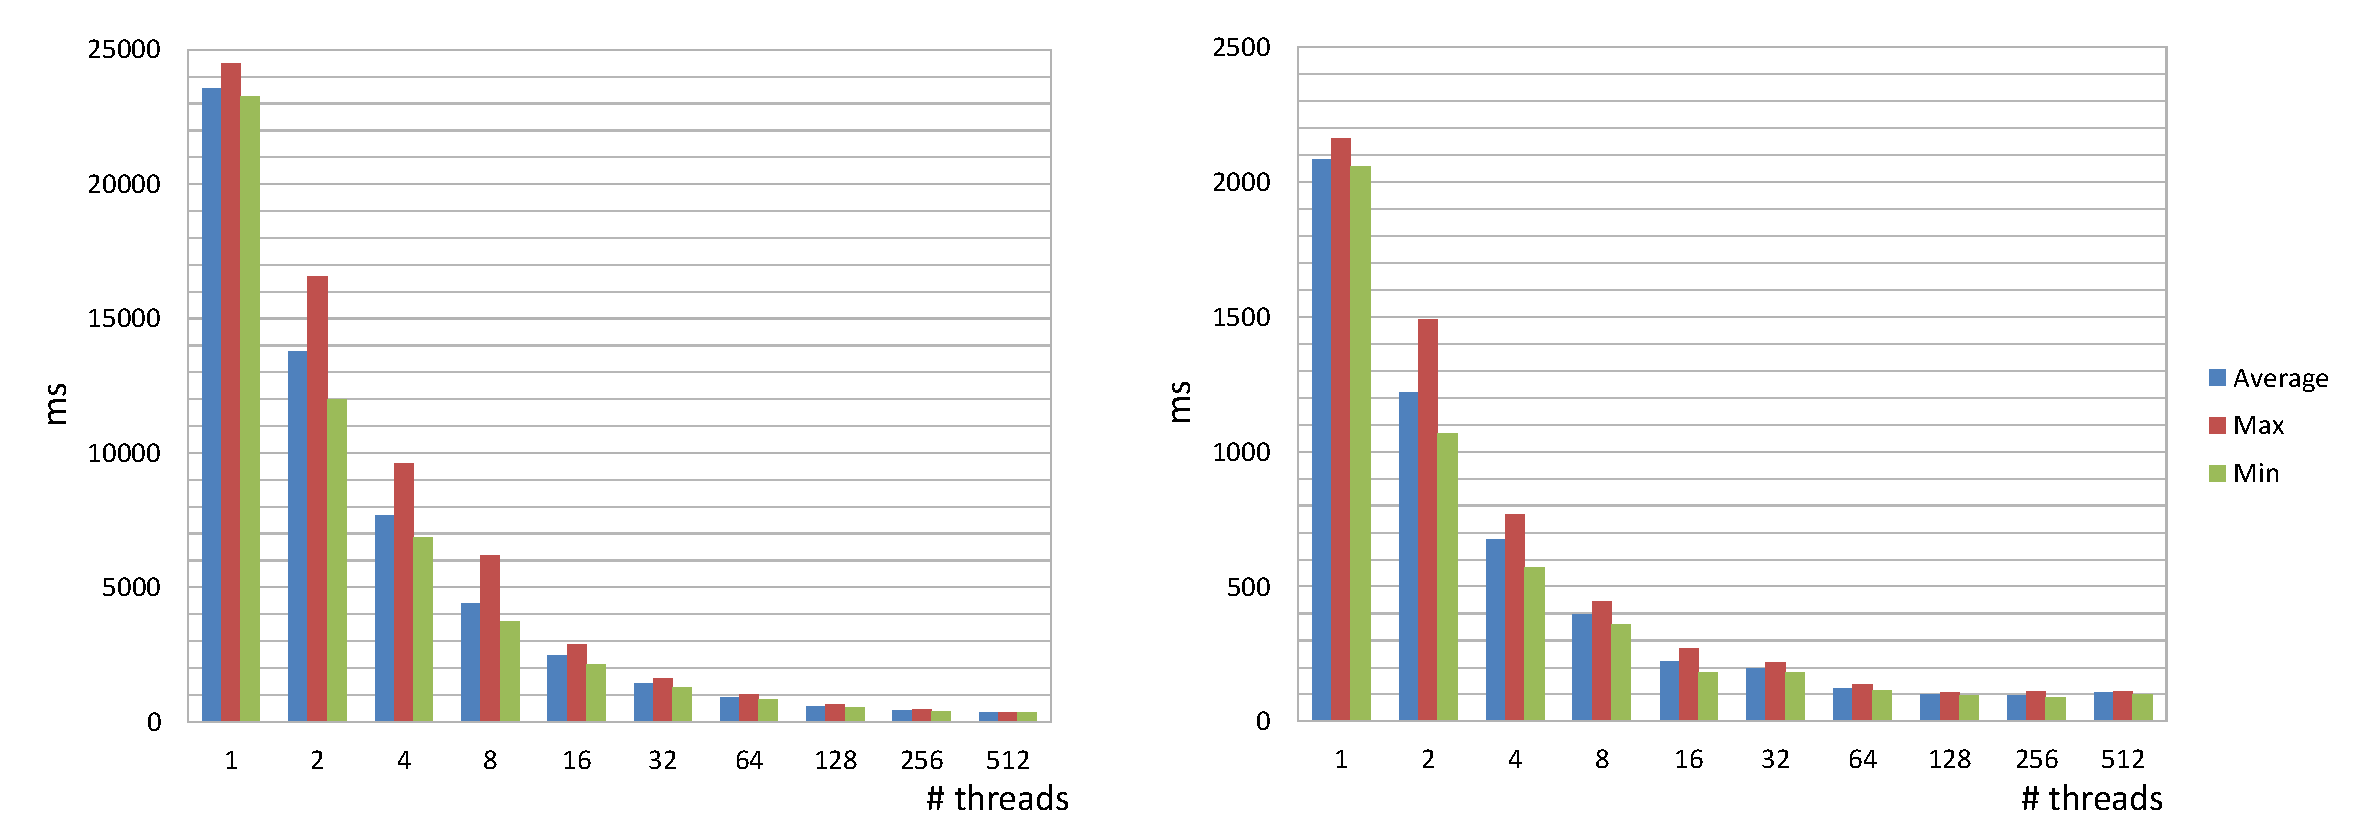
\includegraphics[width=\textwidth]{img/mpi_results.pdf}
	\caption{Runtime results of the MPI implementation for $n=10^{8}$ (left) and $n=10^{7}$ (right).}
\end{figure}
\begin{figure}[h]
	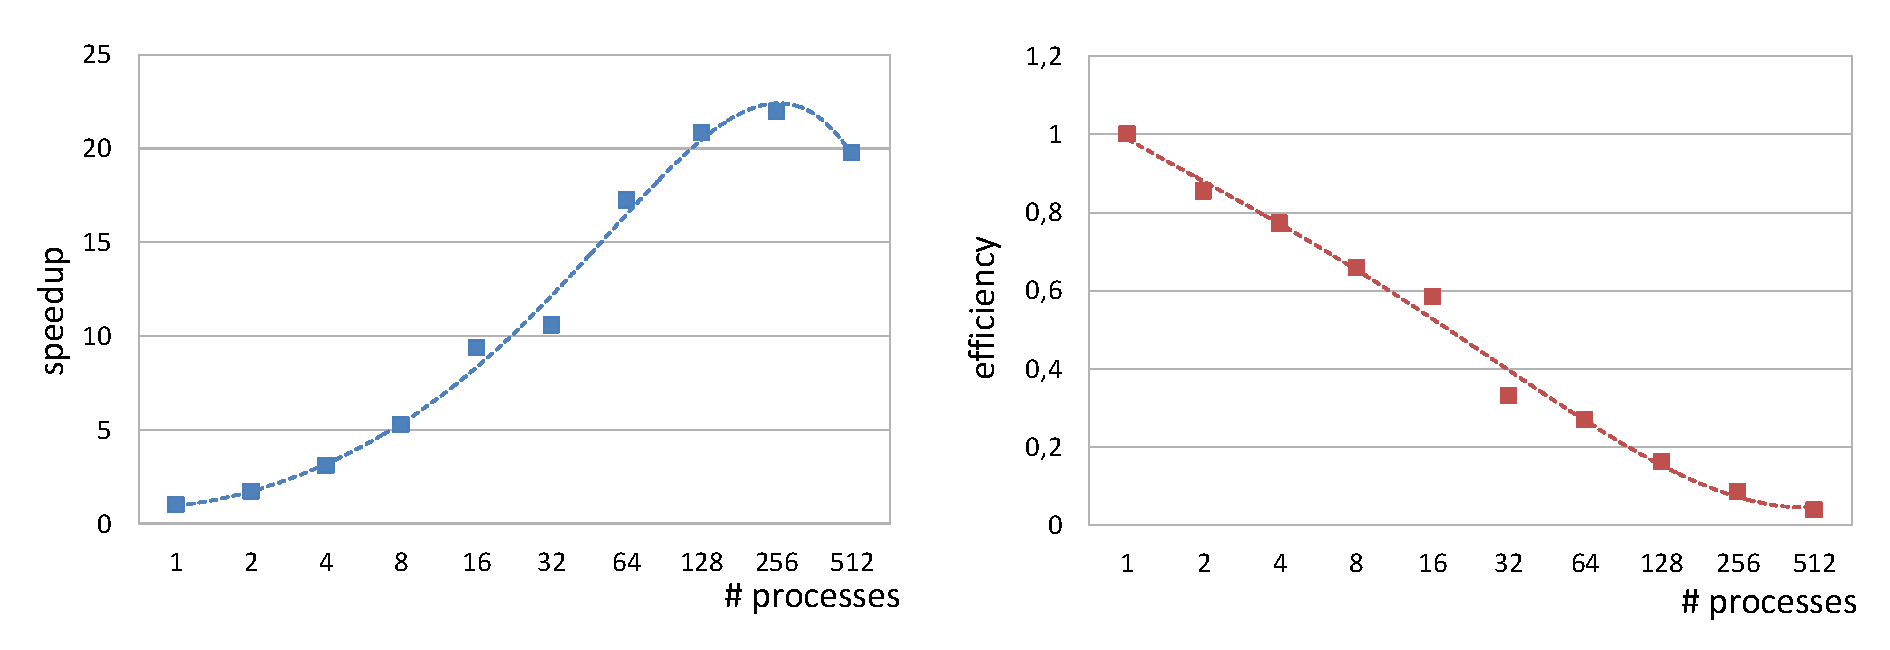
\includegraphics[width=\textwidth]{img/mpi_results_sp_eff10.pdf}
	\caption{Speedup and efficiency results of the MPI implementation for $n=10^{7}$.}
\end{figure}
\begin{figure}[h]
	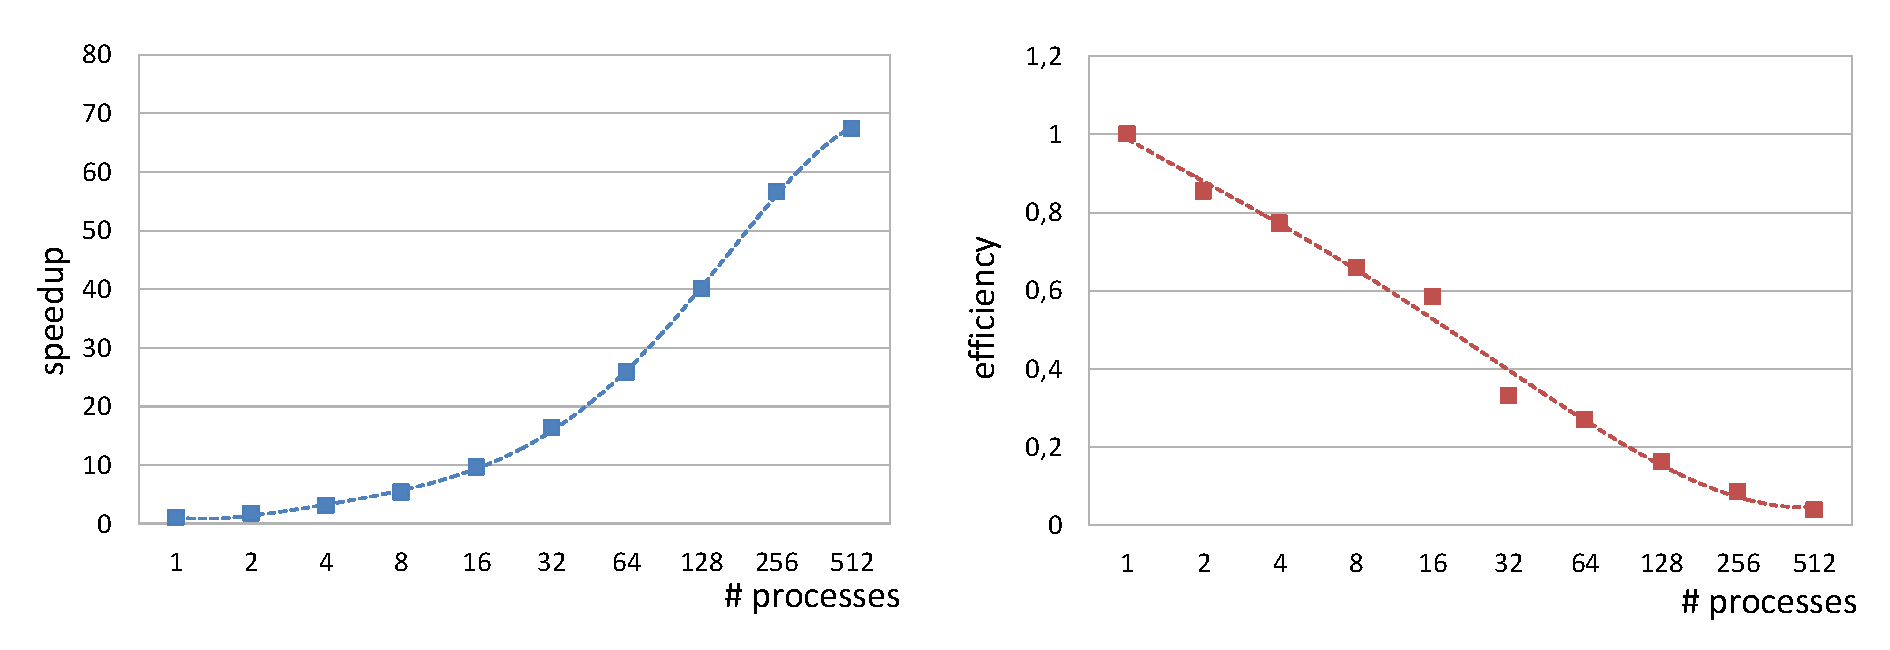
\includegraphics[width=\textwidth]{img/mpi_results_sp_eff100.pdf}
	\caption{Speedup and efficiency results of the MPI implementation for $n=10^{8}$.}
\end{figure}
\begin{figure}[h]
	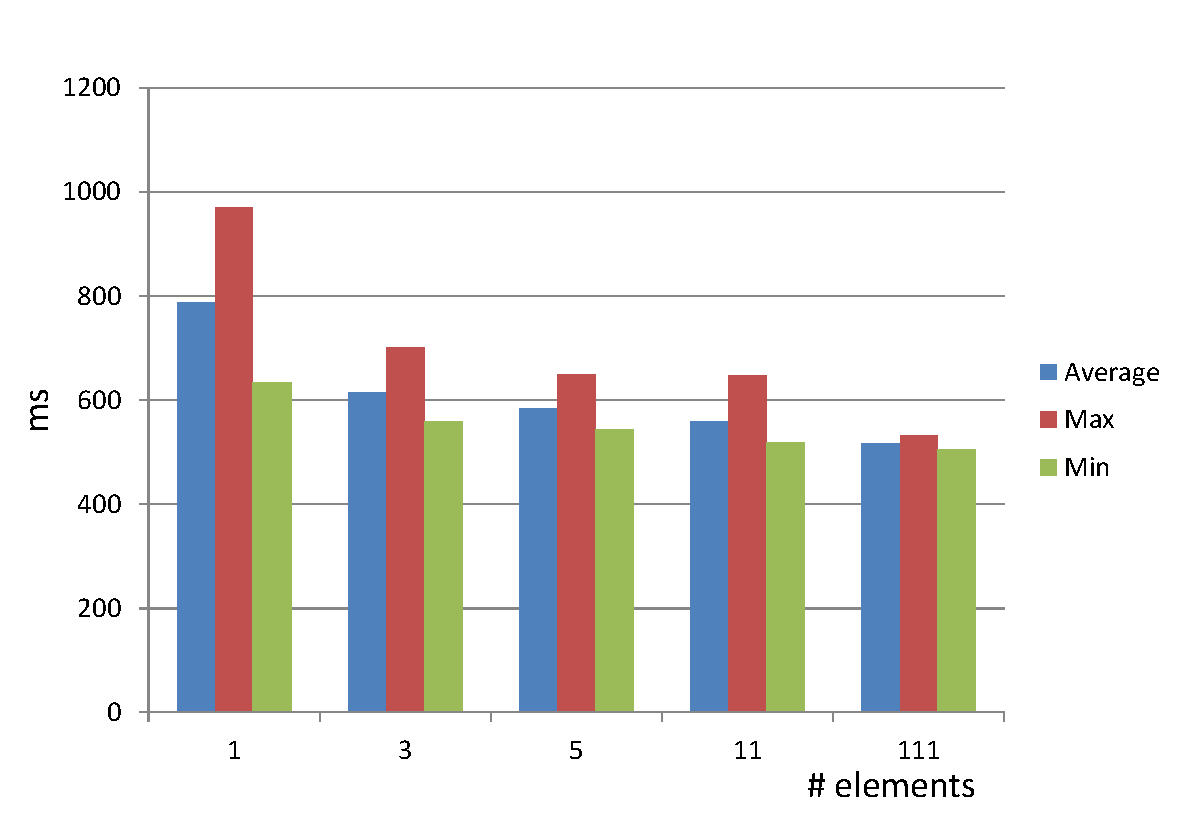
\includegraphics[width=0.7\textwidth]{img/mpi_pivot.pdf}
	\caption{Runtime for $n=10^{8}$ and 128 nodes, different number of elements to compute pivot.}
\end{figure}
\section{Conclusion}

\end{document}
